\section[Introduction to Languages]{Introduction to Languages}
Front End languages are language that are used to give better user experince and user interface. These mainly include HTML, CSS, Javascript. Some Frameforks like Bootstrap are also used with these basic languages.
\subsection{HTML}
\begin{figure}[!ht]
\centering

\includegraphics[width=0.3\textwidth]{input/images/HTML.png}                   
\caption{HTML5 Logo}
\hspace{-1.5em}
\end{figure}
HyperText Markup Language, commonly referred to as HTML, is the standard markup language used to create web pages. Along with CSS, and JavaScript, HTML is a cornerstone technology, used by most websites to create visually engaging webpages, user interfaces for web applications, and user interfaces for many mobile applications. Web browsers can read HTML files and render them into visible or audible web pages. HTML describes the structure of a website semantically along with cues for presentation, making it a markup language, rather than a programming language.


HTML elements form the building blocks of all websites. HTML allows images and objects to be embedded and can be used to create interactive forms. It provides a means to create structured documents by denoting structural semantics for text such as headings, paragraphs, lists, links, quotes and other items.

\begin{verbatim}
<!DOCTYPE html>
<html>
  <head>
    <title>This is a title</title>
  </head>
  <body>
    <p>Hello world!</p>
  </body>
</html>

\end{verbatim}


\subsection{CSS}

\begin{figure}[!ht]
\centering
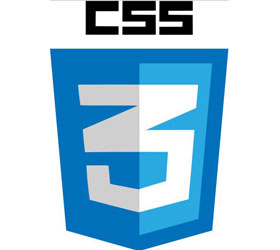
\includegraphics[width=0.3\textwidth]{input/images/CSS.jpg}                   
	\caption{CSS3}
\hspace{-1.5em}
\end{figure}
Cascading Style Sheets (CSS) is a style sheet language used for describing the presentation of a document written in a markup language.Although most often used to set the visual style of web pages and user interfaces written in HTML and XHTML, the language can be applied to any XML document, including plain XML, SVG and XUL, and is applicable to rendering in speech, or on other media. Along with HTML and JavaScript, CSS is a cornerstone technology used by most websites to create visually engaging webpages, user interfaces for web applications, and user interfaces for many mobile applications.


CSS is desgned primarily to enable the separation of document content from document presentation, including aspects such as the layout, colors, and fonts. This separation can improve content accessibility, provide more flexibility and control in the specification of presentation characteristics, enable multiple HTML pages to share formatting by specifying the relevant CSS in a separate .css file, and reduce complexity and repetition in the structural content, such as semantically insignificant tables that were widely used to format pages before consistent CSS rendering was available in all major browsers. CSS makes it possible to separate presentation instructions from the HTML content in a separate file or style section of the HTML file. For each matching HTML element, it provides a list of formatting instructions

\begin{verbatim}
p {
    color: red;
    text-align: center;
} 
\end{verbatim}
\begin{figure}[!ht]
\centering

\includegraphics[width=0.3\textwidth]{input/images/JS.png}
\caption{Javascript}
\hspace{-1.5em}
\end{figure}

JavaScript (/ˈdʒɑːvəˌskrɪpt/) is a high-level, dynamic, untyped, and interpreted programming language. It has been standardized in the ECMAScript language specification. Alongside HTML and CSS, it is one of the three essential technologies of World Wide Web content production; the majority of websites employ it and it is supported by all modern web browsers without plug-ins. JavaScript is prototype-based with first-class functions, making it a multi-paradigm language, supporting object-oriented, imperative, and functional programming styles. It has an API for working with text, arrays, dates and regular expressions, but does not include any I/O, such as networking, storage or graphics facilities, relying for these upon the host environment in which it is embedded.


\begin{figure}[!ht]
	\centering
	
\includegraphics[width=0.3\textwidth]{input/images/bootstrap.png}
	\caption{Bootstrap}
	\hspace{-1.5em}
\end{figure}

Bootstrap is a free and open-source collection of tools for creating websites and web applications. It
contains HTML and CSS-based design templates for typography, forms, buttons, navigation and other
interface components, as well as optional JavaScript extensions.\\
It aims to ease the development of dynamic websites and web applications.\\
Bootstrap is a front end framework, that is, an interface for the user, unlike the server-side code which
resides on the "back end" or server.


\iffalse
\subsection{PHP}
\begin{figure}[!ht]
\centering

\includegraphics[width=0.3\textwidth]{input/images/php.png}
\caption{PHP}
\hspace{-1.5em}
\end{figure}
 {\bf What is PHP?}

    PHP is an acronym for "PHP: Hypertext Preprocessor"
    PHP is a widely-used, open source scripting language
    PHP scripts are executed on the server
    PHP is free to download and use

 {\bf What is a PHP File?}

    PHP files can contain text, HTML, CSS, JavaScript, and PHP code
    PHP code are executed on the server, and the result is returned to the browser as plain HTML
    PHP files have extension ".php"

 {\bf What Can PHP Do?}

    PHP can generate dynamic page content
    PHP can create, open, read, write, delete, and close files on the server
    PHP can collect form data
    PHP can send and receive cookies
    PHP can add, delete, modify data in your database
    PHP can be used to control user-access
    PHP can encrypt data

  {\bf Why PHP?}

    PHP runs on various platforms (Windows, Linux, Unix, Mac OS X, etc.)
    PHP is compatible with almost all servers used today (Apache, IIS, etc.)
    PHP supports a wide range of databases
    PHP is free. Download it from the official PHP resource: www.php.net
    PHP is easy to learn and runs efficiently on the server side
\fi
\subsection{CMake}

CMake is a language(for generator of build systems) with abstract build rules and gnu make is a dependency resolves that executes programs. Cmake takes information on how to build programs generates makefiles that build the program. 

Simple Program 

\begin{figure}[!ht]
\centering
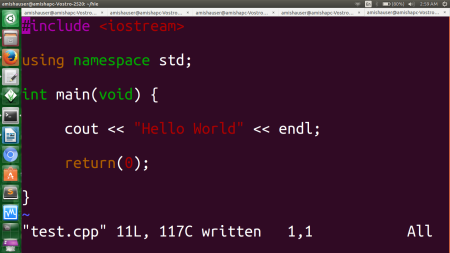
\includegraphics[width=0.6\textwidth]{input/images/cgs/hello.png}                   
\caption{test.cpp file}
\hspace{-1.5em}
\end{figure}

\begin{figure}[!ht]
\centering
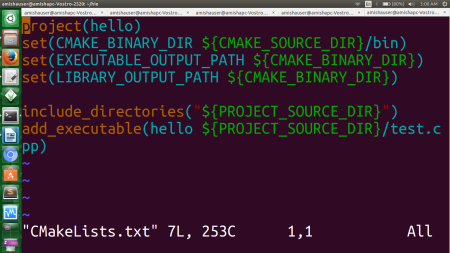
\includegraphics[width=0.6\textwidth]{input/images/cgs/cm.png}                   
\caption{cmake file}
\hspace{-1.5em}
\end{figure}

\subsection{Shell Scripting}
A shell script is a text file that contains a sequence of commands for a UNIX-based operating system. It's called a shell script because it combines into a "script" in a single file a sequence of commands that would otherwise have to be presented to the system from a keyboard one at a time. The shell is the operating system's command interpreter and the set of commands you use to communicate with the system. A shell script is usually created for command sequences for which a user has a repeated need. You initiate the sequence of commands in the shell script by simply entering the name of the shell script on a command line.
\begin{enumerate}
\item Shell script can take input from user or file and output them on screen.
\item Useful to create our own commands.
\item Save lots of time.
\item To automate the task of day to day life.
\item System Administration part can be also automated.
\end{enumerate}
{ \bf Execute your script as syntax:}
\begin{verbatim}
chmod 755 your-script-name
sh your-script-name
./your-script-name
\end{verbatim}

\subsection{Python}
\begin{figure}[h]
	\centering 
\includegraphics[scale=0.3]{input/images/python.png}
	\caption{Python}
\end{figure}
\noindent Python is a dynamic language, as in python coding is very easy and 
also it require less coding and about its interpreted nature it is 
just exellent. Python is a high level programming language and Django 
which is a web development framework is written in python language.

Python is an easy to learn, powerful programming language.Python runs 
on Windows, Linux/Unix, Mac OS X. Python is free to use, even for 
commercial products. Python can also be used as an extension language 
for existing modules and applications that need a programmable interface.  
Python is free to use, even for commercial products, because of its 
OSI-approved open source license.
\subsection{Features of Python}
\begin{itemize}
	\item Very clear, readable syntax.
	\item Strong introspection capabilities.
	\item Intuitive object orientation.

\end{itemize}

